%----------------------------------------------------------------
%
%  File    :  survey-images.tex
%
%  Author  :  Keith Andrews, IICM, TU Graz, Austria
% 
%  Created :  27 May 1993
% 
%  Changed :  03 Feb 2017
% 
%----------------------------------------------------------------


\chapter{Image magnification}

\label{chap:images}

In this part of project we have done following enhancements to our task. We have added zoom feature, which opens picture in new window. The functions, which we implemented work on many different picture formats like svg, jpeg, gif and png.Our enhancements give better possibility for users to see detailed part of image, when they zoom it in, and to see whole picture, without details, when they zoom it out.
\begin{figure}[hp]
\centering

\subcaptionbox[Realy image size in slides ]{%
Realy size of image in slides%
  
    \label{subfig:realy_img}%
}
[%
    0.44\hsize % width of caption
]%
{%
    \includegraphics[keepaspectratio,width=0.225\hsize]%
    {images/image1.png}%
}%
\hspace{0.1\hsize} % seperation
\subcaptionbox[image exxample] {%
   One part of image in after popup window%
    \label{}%
}
[%
    0.44\hsize % width of caption
]%
{%
    \includegraphics[keepaspectratio,width=0.45\hsize]%
    {images/image2.png}%
}%
\caption[]{Screenshot of realy size image and after pop up window. 
\imgcredit{Screenshot taken by the authors of rslide project.
\label{fig:popup}
}}

\end{figure}

\newpage In popup window we can zoom it for +-10\%, +-100\%, and +-1000\%. We can also zoom it with +/- buttons on the keyboard. To switch it in default state, where zoom is 100\%, we can do it with the press of button 0 on the keyboard.
\begin{figure}[tp]
\centering
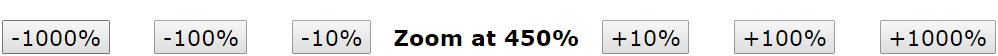
\includegraphics[keepaspectratio,scale=0.5]{images/button.png}

\caption[Buttons function in popup window]{
Buttons function in popup window
\imgcredit{Screenshot taken by the authors of this survey.}

}
\label{fig:Buttons}
\end{figure}

 
On click on image we selected one image and open new window, to which we supply content through javascript document.write function.
\begin{lstlisting}[
language=JavaScript,
label=imposJS,
caption={[Implementetion of select of image in JS]%
In this function we implements a detection and selection one image in slides and open her in new window.
}
]
	  // Input listeners
		var images = document.getElementsByTagName("img");
		var images  = content_section.getElementsByTagName("img");

		for (var i=0, len=images.length, img; i<len; i++) {
		  img = images[i];
		  img.addEventListener("click", function() {
			openImageTab(this.src);
		  });
		}
	};
}

function openImageTab(imgSrc) {
	var newWindow = window.open();
	
	var htmlCode ="<head><title>rSlidy Image View</title><link rel='stylesheet' href='css/reset.css'><link rel='stylesheet' href='css/normalise.css'>" +
			"<link rel='stylesheet' href='css/rslidy.css'><link rel='stylesheet' href='css/slides-default.css'></head>" +
			"<body><div class='slide imageAlert'><h1><button>-1000\%</button><button>-100\%</button><button>-10\%</button>Zoom at <span id='zoomNumber'>100</span>\%<button>+10\%</button><button>+100\%</button><button>+1000\%</button></h1>" +
			"<div><img id='zoomedImg' src='"+ imgSrc + "'></div></div>"+
			"<script type='text/javascript'>" + String(openImageTabListeners) + "; openImageTabListeners();</script></body>";
	newWindow.document.write(htmlCode);
}
\end{lstlisting}

\newpage In content we describe the page layout with buttons, picture, and javascript, which is needed for image resizing.

\begin{lstlisting}[
language=JavaScript,
label=imposJS,
caption={[Implementetion of function for image resizing]%
In this function we implements a image resizing in zoom function.
}
]
	
	window.addEventListener('keypress', function (e) {
		if (e.key == '+' || e.key == '-' || e.key == '0') {
			var zoom = parseInt(titleElement.innerHTML);
			if(e.key == '+'){
				zoom = zoom + 10;
			}
			else if(e.key == '-')
			{
				zoom = zoom - 10;
			}
			else{
				zoom = 100;
			}
			if(zoom > 0){
				img.style.height = zoom * heightPer + "px";
				img.style.width = zoom * widthPer + "px";
				titleElement.innerHTML = zoom;
			}
		}
	}, false);

	var isCtrl = false;
	window.addEventListener('keydown', function (e) {
		if (e.which === 17) {
            isCtrl = true;
        }
    }, false);
	window.addEventListener('keyup', function (e) {
		if (e.which === 17) {
            isCtrl = false;
        }
    }, false);

	window.addEventListener("mousewheel", function (e) {
		if(isCtrl){
			var delta = Math.max(-1, Math.min(1, e.wheelDelta));
			var zoom = parseInt(titleElement.innerHTML);
			if(delta > 0){
				zoom = zoom + 10;
			}
			else if(delta < 0)
			{
				zoom = zoom - 10;
			}
			if(zoom > 0){
				img.style.height = zoom * heightPer + "px";
				img.style.width = zoom * widthPer + "px";
				titleElement.innerHTML = zoom;
			}
		}
	}, false);
}
\end{lstlisting}